% Options for packages loaded elsewhere
% Options for packages loaded elsewhere
\PassOptionsToPackage{unicode}{hyperref}
\PassOptionsToPackage{hyphens}{url}
%
\documentclass[
  ignorenonframetext,
  aspectratio=169,
  russian,
]{beamer}
\newif\ifbibliography
\usepackage{pgfpages}
\setbeamertemplate{caption}[numbered]
\setbeamertemplate{caption label separator}{: }
\setbeamercolor{caption name}{fg=normal text.fg}
\beamertemplatenavigationsymbolshorizontal
% remove section numbering
\setbeamertemplate{part page}{
  \centering
  \begin{beamercolorbox}[sep=16pt,center]{part title}
    \usebeamerfont{part title}\insertpart\par
  \end{beamercolorbox}
}
\setbeamertemplate{section page}{
  \centering
  \begin{beamercolorbox}[sep=12pt,center]{section title}
    \usebeamerfont{section title}\insertsection\par
  \end{beamercolorbox}
}
\setbeamertemplate{subsection page}{
  \centering
  \begin{beamercolorbox}[sep=8pt,center]{subsection title}
    \usebeamerfont{subsection title}\insertsubsection\par
  \end{beamercolorbox}
}
% Prevent slide breaks in the middle of a paragraph
\widowpenalties 1 10000
\raggedbottom
\AtBeginPart{
  \frame{\partpage}
}
\AtBeginSection{
  \ifbibliography
  \else
    \frame{\sectionpage}
  \fi
}
\AtBeginSubsection{
  \frame{\subsectionpage}
}
\usepackage{iftex}
\ifPDFTeX
  \usepackage[T1]{fontenc}
  \usepackage[utf8]{inputenc}
  \usepackage{textcomp} % provide euro and other symbols
\else % if luatex or xetex
  \usepackage{unicode-math} % this also loads fontspec
  \defaultfontfeatures{Scale=MatchLowercase}
  \defaultfontfeatures[\rmfamily]{Ligatures=TeX,Scale=1}
\fi
\usepackage{lmodern}

\ifPDFTeX\else
  % xetex/luatex font selection
\fi
% Use upquote if available, for straight quotes in verbatim environments
\IfFileExists{upquote.sty}{\usepackage{upquote}}{}
\IfFileExists{microtype.sty}{% use microtype if available
  \usepackage[]{microtype}
  \UseMicrotypeSet[protrusion]{basicmath} % disable protrusion for tt fonts
}{}


\usepackage{longtable,booktabs,array}
\newcounter{none} % for unnumbered tables
\usepackage{calc} % for calculating minipage widths
\usepackage{caption}
% Make caption package work with longtable
\makeatletter
\def\fnum@table{\tablename~\thetable}
\makeatother
\usepackage{graphicx}
\makeatletter
\newsavebox\pandoc@box
\newcommand*\pandocbounded[1]{% scales image to fit in text height/width
  \sbox\pandoc@box{#1}%
  \Gscale@div\@tempa{\textheight}{\dimexpr\ht\pandoc@box+\dp\pandoc@box\relax}%
  \Gscale@div\@tempb{\linewidth}{\wd\pandoc@box}%
  \ifdim\@tempb\p@<\@tempa\p@\let\@tempa\@tempb\fi% select the smaller of both
  \ifdim\@tempa\p@<\p@\scalebox{\@tempa}{\usebox\pandoc@box}%
  \else\usebox{\pandoc@box}%
  \fi%
}
% Set default figure placement to htbp
\def\fps@figure{htbp}
\makeatother



\ifLuaTeX
\usepackage[bidi=basic,shorthands=off,provide=*]{babel}
\else
\usepackage[bidi=default,shorthands=off,provide=*]{babel}
\fi
\ifLuaTeX
  \usepackage{selnolig} % disable illegal ligatures
\fi


\setlength{\emergencystretch}{3em} % prevent overfull lines

\providecommand{\tightlist}{%
  \setlength{\itemsep}{0pt}\setlength{\parskip}{0pt}}



 

\usepackage[]{csquotes}

\IfFileExists{plex-otf.sty}{
  %% Full TeXlive
  % \usepackage[%
  %   % math,
  %   RM={Scale=0.94},SS={Scale=0.94},SScon={Scale=0.94},TT={Scale=MatchLowercase,FakeStretch=0.9},DefaultFeatures={Ligatures=Common}
  % ]{plex-otf}
}{
  %% TinyTeX
  \usepackage{libertine}
}

%%% Load theme
% https://deic.uab.cat/~iblanes/beamer_gallery/
\IfFileExists{beamerthemegotham.sty}{
  %% Full TeXlive
  \usetheme{gotham}
  \gothamset{
    numbering=totalpagenumber,
    parttocframe default=off,
    sectiontocframe default=off,
    subsectiontocframe default=off,
  }
}{
  %% TinyTeX
  \usetheme{Madrid}
}
\makeatletter
\@ifpackageloaded{caption}{}{\usepackage{caption}}
\AtBeginDocument{%
\ifdefined\contentsname
  \renewcommand*\contentsname{Содержание}
\else
  \newcommand\contentsname{Содержание}
\fi
\ifdefined\listfigurename
  \renewcommand*\listfigurename{Список иллюстраций}
\else
  \newcommand\listfigurename{Список иллюстраций}
\fi
\ifdefined\listtablename
  \renewcommand*\listtablename{Список таблиц}
\else
  \newcommand\listtablename{Список таблиц}
\fi
\ifdefined\figurename
  \renewcommand*\figurename{Рисунок}
\else
  \newcommand\figurename{Рисунок}
\fi
\ifdefined\tablename
  \renewcommand*\tablename{Таблица}
\else
  \newcommand\tablename{Таблица}
\fi
}
\@ifpackageloaded{float}{}{\usepackage{float}}
\floatstyle{ruled}
\@ifundefined{c@chapter}{\newfloat{codelisting}{h}{lop}}{\newfloat{codelisting}{h}{lop}[chapter]}
\floatname{codelisting}{Список}
\newcommand*\listoflistings{\listof{codelisting}{Листинги}}
\makeatother
\makeatletter
\makeatother
\makeatletter
\@ifpackageloaded{caption}{}{\usepackage{caption}}
\@ifpackageloaded{subcaption}{}{\usepackage{subcaption}}
\makeatother

\usepackage{bookmark}
\IfFileExists{xurl.sty}{\usepackage{xurl}}{} % add URL line breaks if available
\urlstyle{same}
% fallback for those not using the hyperref driver hyperxmp:
\makeatletter
\@ifundefined{xmpquote}{\newcommand{\xmpquote}[1]{#1}}{}
\makeatother
\hypersetup{
  pdftitle={Лабораторная работа №3},
  pdfauthor={Кудякова София Андреевна},
  pdflang={ru},
  hidelinks,
  pdfcreator={LaTeX via pandoc}}


\title{\texorpdfstring{Лабораторная работа №3}{Лабораторная работа №3}}
\subtitle{\texorpdfstring{Агентное
моделирование}{Агентное моделирование}}
\author{Кудякова София Андреевна}
\date{2026-08-27}

\begin{document}
\frame{\titlepage}

\renewcommand*\contentsname{Содержание}
\begin{frame}[allowframebreaks]
  \frametitle{Содержание}
  \setcounter{tocdepth}{1}
  \tableofcontents
\end{frame}
\setcounter{tocdepth}{1}
\tableofcontents
}

\section{Вводная
часть}\label{ux432ux432ux43eux434ux43dux430ux44f-ux447ux430ux441ux442ux44c}

\begin{frame}{Цель и задачи}
\protect\phantomsection\label{ux446ux435ux43bux44c-ux438-ux437ux430ux434ux430ux447ux438}
\textbf{Цель:} познакомиться с агентным подходом к имитационному
моделированию, реализовать модель DaisyWorld на Julia и исследовать
влияние параметров модели.

\textbf{Задачи:}

\begin{itemize}[<+->]
\tightlist
\item
  реализовать модель DaisyWorld;
\item
  преобразовать код в литературный стиль;
\item
  сгенерировать Julia-код, Jupyter Notebook и документ Quarto;
\item
  реализовать визуализацию и анимацию;
\item
  исследовать динамику численности маргариток;
\item
  исследовать влияние солнечной светимости;
\item
  выполнить параметрическое исследование.
\end{itemize}
\end{frame}

\begin{frame}{Агентное моделирование}
\protect\phantomsection\label{ux430ux433ux435ux43dux442ux43dux43eux435-ux43cux43eux434ux435ux43bux438ux440ux43eux432ux430ux43dux438ux435}
Подход, при котором система представляется как совокупность
взаимодействующих автономных агентов.

Основные элементы:

\begin{itemize}[<+->]
\tightlist
\item
  \textbf{агенты} --- автономные объекты со своими свойствами;
\item
  \textbf{среда} --- пространство, в котором находятся агенты;
\item
  \textbf{правила взаимодействия} --- определяют изменение состояния
  агентов и среды.
\end{itemize}
\end{frame}

\begin{frame}{Модель DaisyWorld}
\protect\phantomsection\label{ux43cux43eux434ux435ux43bux44c-daisyworld}
Агентная модель взаимодействия чёрных и белых маргариток со средой.

\begin{itemize}[<+->]
\tightlist
\item
  чёрные маргаритки --- меньшее альбедо, поглощают больше излучения;
\item
  белые маргаритки --- отражают больше излучения, охлаждают среду;
\item
  среда --- двумерная сетка с температурой в каждой клетке;
\item
  агенты стареют, погибают и размножаются.
\end{itemize}

Изменение численности маргариток влияет на температуру, а температура
--- на дальнейшую динамику популяций.
\end{frame}

\section{Подготовка
проекта}\label{ux43fux43eux434ux433ux43eux442ux43eux432ux43aux430-ux43fux440ux43eux435ux43aux442ux430}

\begin{frame}[fragile]{Структура проекта}
\protect\phantomsection\label{ux441ux442ux440ux443ux43aux442ux443ux440ux430-ux43fux440ux43eux435ux43aux442ux430}
Каталоги: \texttt{scripts}, \texttt{src}, \texttt{markdown},
\texttt{notebooks}, \texttt{plots}, \texttt{data}, \texttt{test}.

\begin{figure}

\centering{


\includegraphics[width=0.7\linewidth,height=\textheight,keepaspectratio]{image/1.png}

}

\caption{\label{fig-001}Структура проекта}

\end{figure}%
\end{frame}

\begin{frame}{Подготовка рабочего окружения}
\protect\phantomsection\label{ux43fux43eux434ux433ux43eux442ux43eux432ux43aux430-ux440ux430ux431ux43eux447ux435ux433ux43e-ux43eux43aux440ux443ux436ux435ux43dux438ux44f}
Установлены необходимые пакеты Julia, выполнена проверка окружения.

\begin{figure}

\centering{


\includegraphics[width=0.7\linewidth,height=\textheight,keepaspectratio]{image/2.png}

}

\caption{\label{fig-002}Проверка рабочего окружения}

\end{figure}%
\end{frame}

\section{Реализация
модели}\label{ux440ux435ux430ux43bux438ux437ux430ux446ux438ux44f-ux43cux43eux434ux435ux43bux438}

\begin{frame}[fragile]{Базовая модель}
\protect\phantomsection\label{ux431ux430ux437ux43eux432ux430ux44f-ux43cux43eux434ux435ux43bux44c}
Реализация в \texttt{src/daisyworld.jl}:

\begin{itemize}[<+->]
\tightlist
\item
  создание агентов;
\item
  расчёт и распространение температуры;
\item
  размножение, старение и гибель маргариток;
\item
  изменение солнечной светимости.
\end{itemize}

\begin{figure}

\centering{


\includegraphics[width=0.7\linewidth,height=\textheight,keepaspectratio]{image/3.png}

}

\caption{\label{fig-003}Результат базового моделирования}

\end{figure}%
\end{frame}

\begin{frame}{Визуализация состояний}
\protect\phantomsection\label{ux432ux438ux437ux443ux430ux43bux438ux437ux430ux446ux438ux44f-ux441ux43eux441ux442ux43eux44fux43dux438ux439}
Сохранены состояния системы на разных шагах моделирования.

\begin{figure}

\centering{


\includegraphics[width=0.7\linewidth,height=\textheight,keepaspectratio]{image/4.png}

}

\caption{\label{fig-004}Состояние модели на различных шагах}

\end{figure}%

\begin{figure}

\centering{

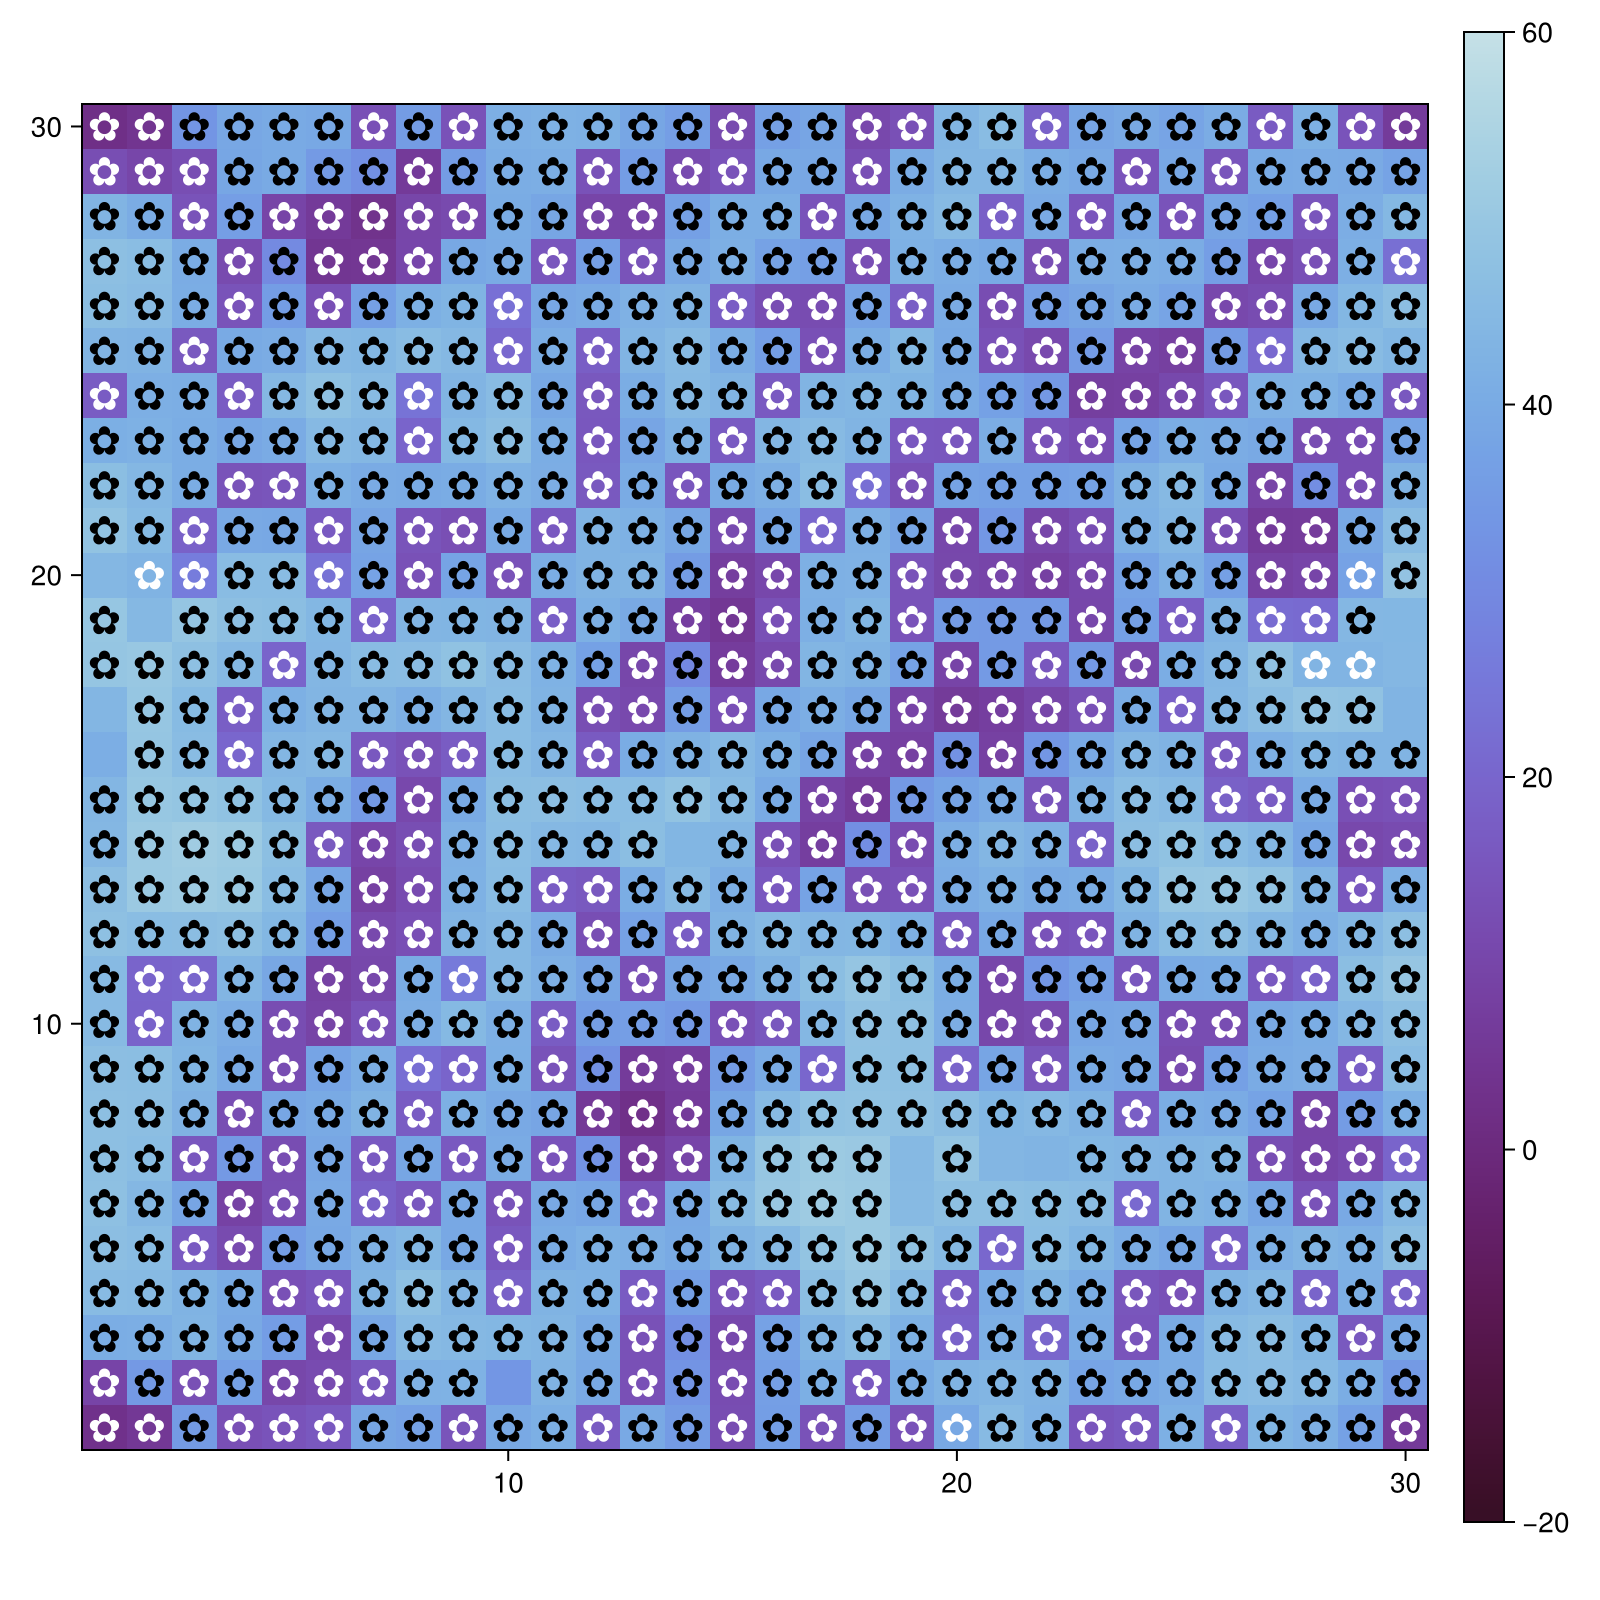
\includegraphics[width=0.7\linewidth,height=\textheight,keepaspectratio]{image/44.png}

}

\caption{\label{fig-044}Состояние модели на различных шагах}

\end{figure}%

\begin{figure}

\centering{

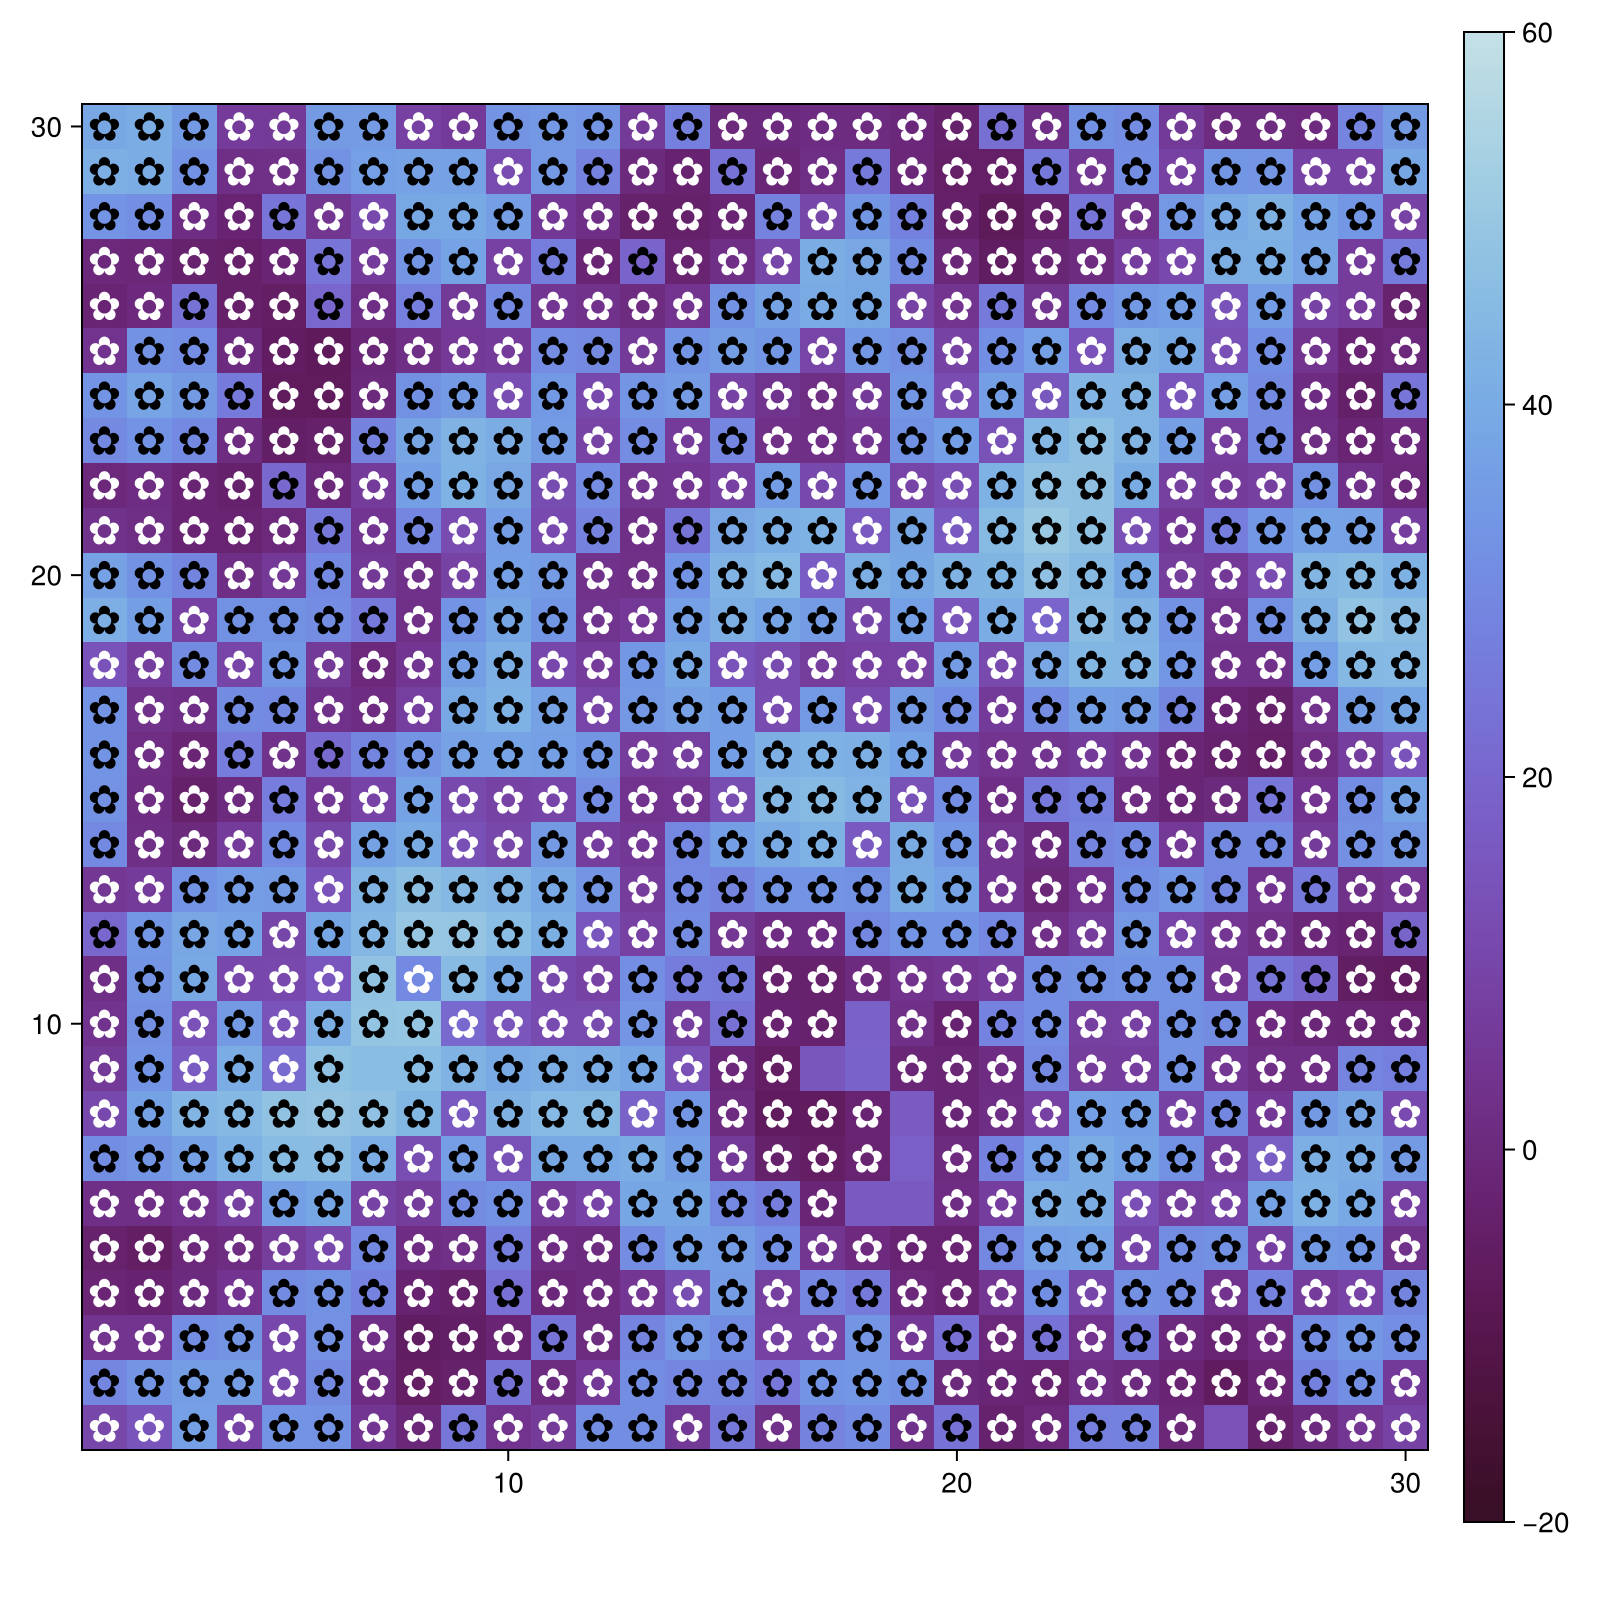
\includegraphics[width=0.7\linewidth,height=\textheight,keepaspectratio]{image/444.png}

}

\caption{\label{fig-444}Состояние модели на различных шагах}

\end{figure}%
\end{frame}

\section{Анимация}\label{ux430ux43dux438ux43cux430ux446ux438ux44f}

\begin{frame}[fragile]{Динамика во времени}
\protect\phantomsection\label{ux434ux438ux43dux430ux43cux438ux43aux430-ux432ux43e-ux432ux440ux435ux43cux435ux43dux438}
Создана анимация модели DaisyWorld --- файл \texttt{simulation.mp4}.

\begin{figure}

\centering{


\includegraphics[width=0.7\linewidth,height=\textheight,keepaspectratio]{image/5.png}

}

\caption{\label{fig-005}Кадр анимации DaisyWorld}

\end{figure}%

Анимация показывает изменение распределения маргариток и температуры
среды во времени.
\end{frame}

\section{Динамика
численности}\label{ux434ux438ux43dux430ux43cux438ux43aux430-ux447ux438ux441ux43bux435ux43dux43dux43eux441ux442ux438}

\begin{frame}{Изменение количества маргариток}
\protect\phantomsection\label{ux438ux437ux43cux435ux43dux435ux43dux438ux435-ux43aux43eux43bux438ux447ux435ux441ux442ux432ux430-ux43cux430ux440ux433ux430ux440ux438ux442ux43eux43a}
Выполнен длительный запуск модели, построен график динамики чёрных и
белых маргариток.

\begin{figure}

\centering{


\includegraphics[width=0.7\linewidth,height=\textheight,keepaspectratio]{image/6.png}

}

\caption{\label{fig-006}Динамика численности маргариток}

\end{figure}%

Динамика популяций определяется взаимодействием агентов со средой и
между собой.
\end{frame}

\section{Изменение солнечной
светимости}\label{ux438ux437ux43cux435ux43dux435ux43dux438ux435-ux441ux43eux43bux43dux435ux447ux43dux43eux439-ux441ux432ux435ux442ux438ux43cux43eux441ux442ux438}

\begin{frame}{Сценарий \texttt{:ramp}}
\protect\phantomsection\label{ux441ux446ux435ux43dux430ux440ux438ux439-ramp}
Солнечная светимость изменяется во времени.

\begin{figure}

\centering{


\includegraphics[width=0.7\linewidth,height=\textheight,keepaspectratio]{image/7.png}

}

\caption{\label{fig-007}Изменение модели при изменении светимости}

\end{figure}%

Изменение светимости меняет условия существования маргариток и влияет на
численность обеих популяций.
\end{frame}

\section{Параметрическое
исследование}\label{ux43fux430ux440ux430ux43cux435ux442ux440ux438ux447ux435ux441ux43aux43eux435-ux438ux441ux441ux43bux435ux434ux43eux432ux430ux43dux438ux435}

\begin{frame}[fragile]{Исследуемые параметры}
\protect\phantomsection\label{ux438ux441ux441ux43bux435ux434ux443ux435ux43cux44bux435-ux43fux430ux440ux430ux43cux435ux442ux440ux44b}
\begin{itemize}[<+->]
\tightlist
\item
  \texttt{max\_age} --- максимальный возраст маргариток;
\item
  \texttt{init\_white} --- начальная доля белых маргариток.
\end{itemize}

\begin{figure}

\centering{


\includegraphics[width=0.7\linewidth,height=\textheight,keepaspectratio]{image/8.png}

}

\caption{\label{fig-008}Параметрические запуски}

\end{figure}%
\end{frame}

\begin{frame}[fragile]{Результаты параметрического исследования}
\protect\phantomsection\label{ux440ux435ux437ux443ux43bux44cux442ux430ux442ux44b-ux43fux430ux440ux430ux43cux435ux442ux440ux438ux447ux435ux441ux43aux43eux433ux43e-ux438ux441ux441ux43bux435ux434ux43eux432ux430ux43dux438ux44f}
\begin{figure}

\centering{


\includegraphics[width=0.7\linewidth,height=\textheight,keepaspectratio]{image/9.png}

}

\caption{\label{fig-009}Результаты параметрического исследования}

\end{figure}%

\begin{figure}

\centering{

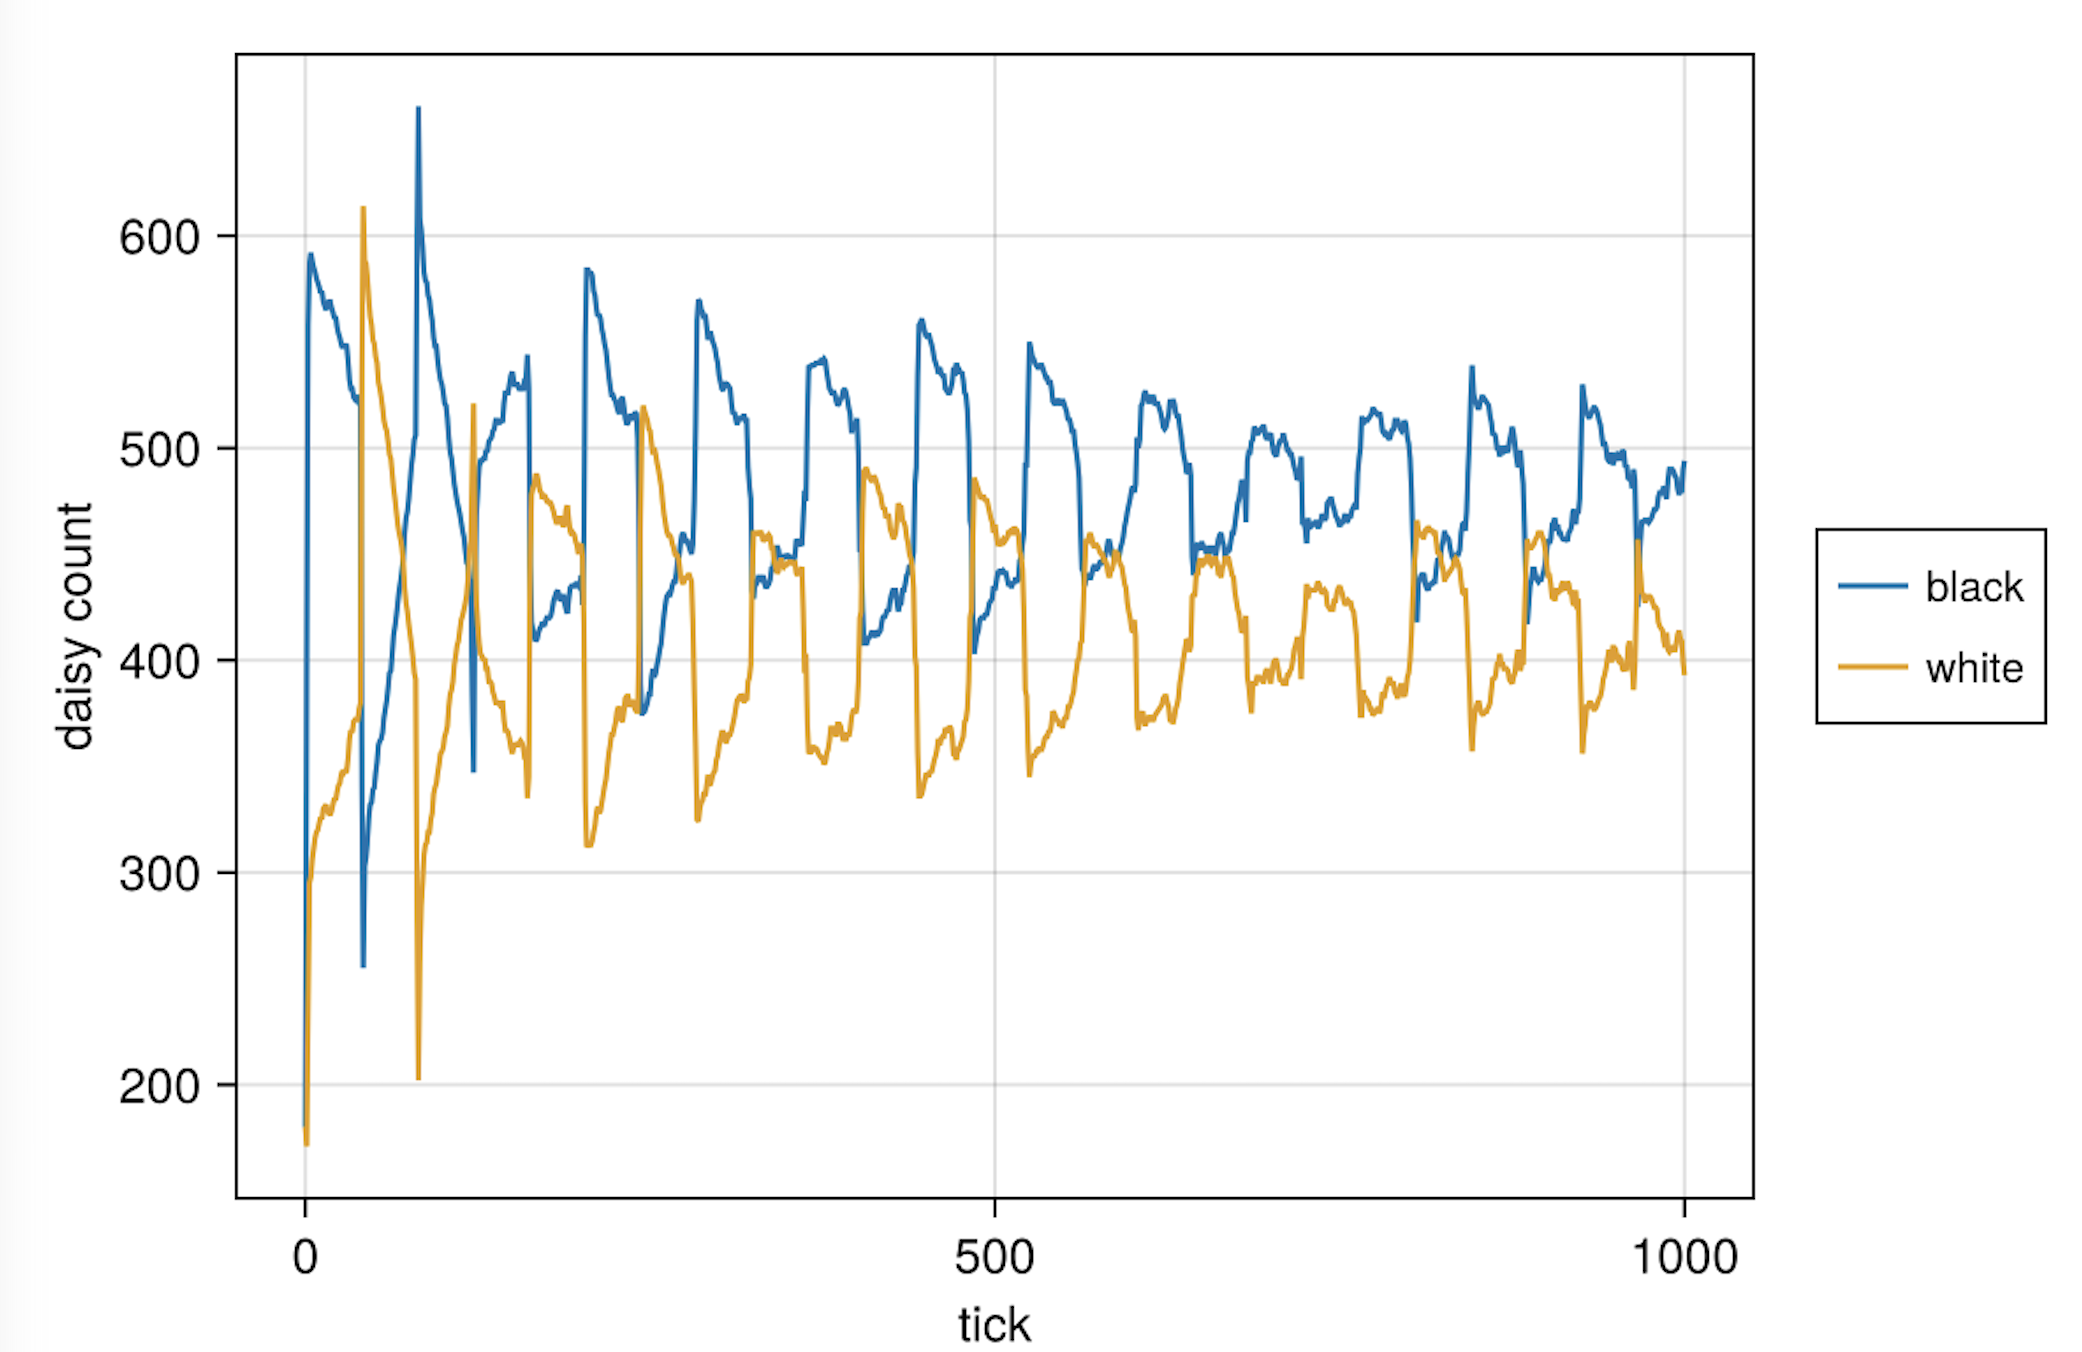
\includegraphics[width=0.7\linewidth,height=\textheight,keepaspectratio]{image/99.png}

}

\caption{\label{fig-099}Результаты параметрического исследования}

\end{figure}%

\begin{itemize}[<+->]
\tightlist
\item
  изменение \texttt{max\_age} влияет на скорость смены поколений;
\item
  изменение \texttt{init\_white} влияет на начальное соотношение
  популяций и дальнейшую динамику.
\end{itemize}
\end{frame}

\begin{frame}{Параметрическое исследование светимости}
\protect\phantomsection\label{ux43fux430ux440ux430ux43cux435ux442ux440ux438ux447ux435ux441ux43aux43eux435-ux438ux441ux441ux43bux435ux434ux43eux432ux430ux43dux438ux435-ux441ux432ux435ux442ux438ux43cux43eux441ux442ux438}
\begin{figure}

\centering{


\includegraphics[width=0.7\linewidth,height=\textheight,keepaspectratio]{image/10.png}

}

\caption{\label{fig-010}Параметрическое исследование светимости}

\end{figure}%

\begin{figure}

\centering{

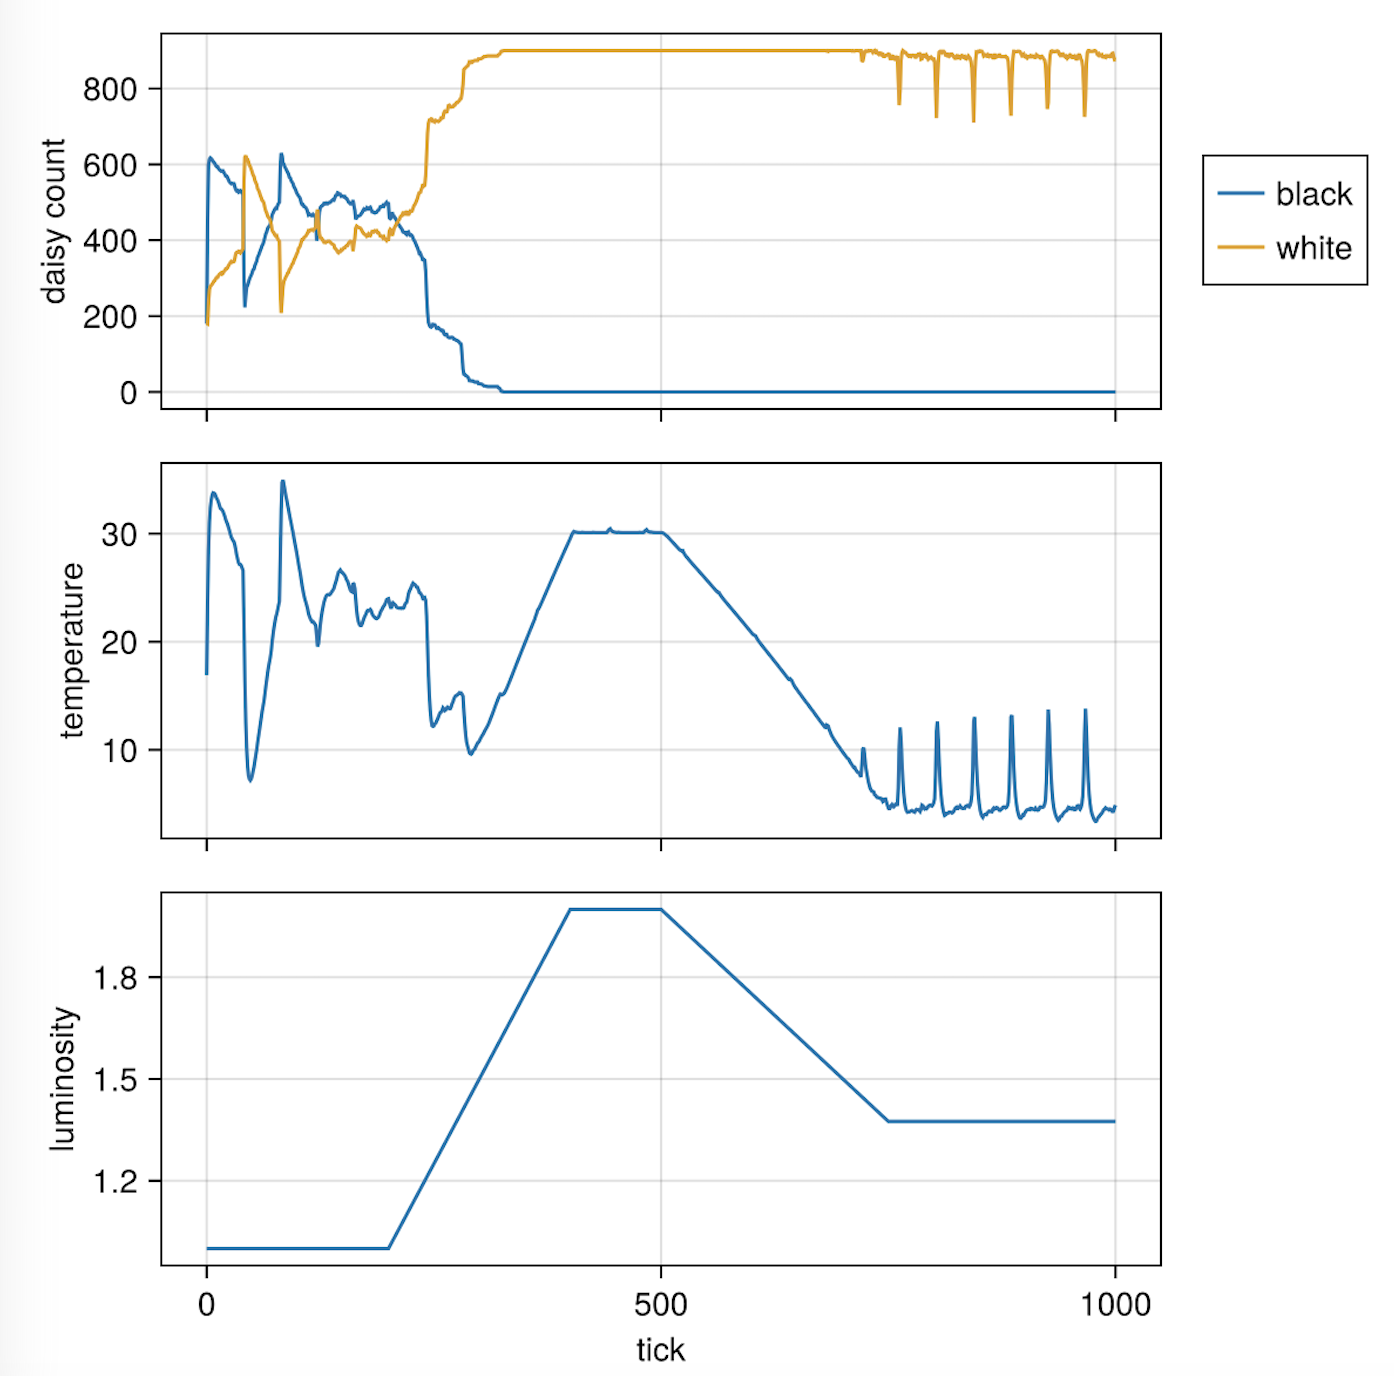
\includegraphics[width=0.7\linewidth,height=\textheight,keepaspectratio]{image/101.png}

}

\caption{\label{fig-101}Параметрическое исследование светимости}

\end{figure}%

Результаты демонстрируют разное поведение системы при изменении
начальных условий и параметров агентов.
\end{frame}

\section{Литературное
программирование}\label{ux43bux438ux442ux435ux440ux430ux442ux443ux440ux43dux43eux435-ux43fux440ux43eux433ux440ux430ux43cux43cux438ux440ux43eux432ux430ux43dux438ux435}

\begin{frame}{Генерация производных файлов}
\protect\phantomsection\label{ux433ux435ux43dux435ux440ux430ux446ux438ux44f-ux43fux440ux43eux438ux437ux432ux43eux434ux43dux44bux445-ux444ux430ux439ux43bux43eux432}
Из литературного кода получены Julia-скрипты, Jupyter Notebook и
документы Quarto.

\begin{figure}

\centering{


\includegraphics[width=0.7\linewidth,height=\textheight,keepaspectratio]{image/11.png}

}

\caption{\label{fig-011}Генерация производных файлов}

\end{figure}%

\begin{figure}

\centering{


\includegraphics[width=0.7\linewidth,height=\textheight,keepaspectratio]{image/12.png}

}

\caption{\label{fig-012}Структура каталогов после генерации}

\end{figure}%
\end{frame}

\section{Jupyter Notebook}\label{jupyter-notebook}

\begin{frame}{Выполнение Notebook}
\protect\phantomsection\label{ux432ux44bux43fux43eux43bux43dux435ux43dux438ux435-notebook}
Сгенерированные Notebook выполнены для проверки воспроизводимости
результатов.

\begin{figure}

\centering{


\includegraphics[width=0.7\linewidth,height=\textheight,keepaspectratio]{image/13.png}

}

\caption{\label{fig-013}Выполнение Jupyter Notebook базовой модели}

\end{figure}%

\begin{figure}

\centering{


\includegraphics[width=0.7\linewidth,height=\textheight,keepaspectratio]{image/14.png}

}

\caption{\label{fig-014}Выполнение Notebook}

\end{figure}%
\end{frame}

\section{Результаты}\label{ux440ux435ux437ux443ux43bux44cux442ux430ux442ux44b}

\begin{frame}{Базовое моделирование}
\protect\phantomsection\label{ux431ux430ux437ux43eux432ux43eux435-ux43cux43eux434ux435ux43bux438ux440ux43eux432ux430ux43dux438ux435}
\begin{itemize}[<+->]
\tightlist
\item
  реализована агентная модель DaisyWorld;
\item
  агенты взаимодействуют со средой;
\item
  учитываются температура, возраст и тип маргариток;
\item
  реализованы размножение и гибель агентов.
\end{itemize}
\end{frame}

\begin{frame}{Динамика и внешние воздействия}
\protect\phantomsection\label{ux434ux438ux43dux430ux43cux438ux43aux430-ux438-ux432ux43dux435ux448ux43dux438ux435-ux432ux43eux437ux434ux435ux439ux441ux442ux432ux438ux44f}
\begin{itemize}[<+->]
\tightlist
\item
  численность чёрных и белых маргариток изменяется во времени;
\item
  различное альбедо влияет на температуру среды;
\item
  изменение солнечной светимости меняет состояние популяций.
\end{itemize}
\end{frame}

\begin{frame}[fragile]{Параметрическое исследование}
\protect\phantomsection\label{ux43fux430ux440ux430ux43cux435ux442ux440ux438ux447ux435ux441ux43aux43eux435-ux438ux441ux441ux43bux435ux434ux43eux432ux430ux43dux438ux435-1}
\begin{itemize}[<+->]
\tightlist
\item
  исследовано влияние \texttt{max\_age} и \texttt{init\_white};
\item
  получены результаты для нескольких комбинаций параметров;
\item
  исследовано поведение модели при изменении светимости.
\end{itemize}
\end{frame}

\section{Выводы}\label{ux432ux44bux432ux43eux434ux44b}

\begin{frame}{Выводы}
\begin{itemize}[<+->]
\tightlist
\item
  изучен агентный подход к имитационному моделированию;
\item
  реализована модель DaisyWorld на Julia;
\item
  выполнена визуализация и создана анимация;
\item
  исследована динамика численности маргариток и влияние светимости;
\item
  выполнено параметрическое исследование;
\item
  реализовано литературное программирование;
\item
  сгенерированы и выполнены Julia-скрипты, Jupyter Notebook и
  Quarto-документы.
\end{itemize}
\end{frame}




\end{document}
